\documentclass[11pt,a4paper]{article}
\usepackage[utf8]{inputenc}
\usepackage[T1]{fontenc}
\usepackage{mathptmx}
\usepackage[margin=2.5cm]{geometry}
\usepackage{graphicx,booktabs,multirow,hyperref,setspace,amsmath,amsfonts}
\usepackage[numbers,sort&compress]{natbib}
\usepackage{caption,subcaption,enumitem}
\usepackage{fancyhdr}
\pagestyle{fancy}\fancyhf{}\fancyhead[R]{\thepage}\renewcommand{\headrulewidth}{0.4pt}
\fancyhead[L]{\small Mahalanobis Distance-Based Biomarker Dysregulation and Residual CV Mortality}
\setlength{\bibsep}{2pt}

\title{\textbf{Mahalanobis distance-based biomarker network dysregulation and residual cardiovascular mortality: a binational cohort study}}

\author{
Qingsong Gong$^{1}$, Yuzhi Fan$^{1}$, Sixuan Shao$^{1}$, Xiaohan Li$^{1}$, Yajing Du$^{1}$, Qingping Guo$^{2,*}$\\
\\
$^{1}$Changzhi Medical College, Changzhi, Shanxi, China\\
$^{2}$Heji Hospital Affiliated to Changzhi Medical College, Changzhi, Shanxi, China\\
\\
$^{*}$Corresponding author: kuijing198ffw@163.com\\
}

\date{}

\begin{document}
\maketitle

\begin{abstract}
\subsection*{Background}
Traditional cardiovascular risk scores miss 18--41\% of individuals who later experience cardiovascular events. Existing composite biomarker indices combine biomarkers through linear formulas that ignore the interdependence among physiological systems and consequently fail to capture multi-system dysregulation. We developed and validated Network-CMIN, a Mahalanobis distance-based measure of biomarker network dysregulation, to predict mortality and reclassify residual risk beyond traditional risk stratification.

\subsection*{Methods}
Binational cohort study. Derivation cohort: China Health and Retirement Longitudinal Study (CHARLS) 2015 wave ($N = 12{,}436$, median follow-up 5.4 years, 852 deaths). External validation cohort: National Health and Nutrition Examination Survey (NHANES) 1999--2016 ($N = 17{,}804$, median follow-up 9.7 years, 3,446 all-cause deaths; 1,012 cardiovascular deaths via NDI linkage). An exploratory CRP-inclusive sub-analysis used NHANES 2015--2016 Wave I ($N = 2{,}349$, 107 deaths). Network-CMIN was calculated as the Mahalanobis distance of each participant's 7--10 routine clinical biomarkers from a healthy reference centroid. The primary outcome was all-cause mortality. Analyses employed Cox proportional hazards models, restricted cubic splines, C-index comparison, and a four-group discordance framework.

\subsection*{Results}
Per 1-SD increase in Network-CMIN, adjusted hazard ratios (HR) for all-cause mortality were 1.14 (95\% CI, 1.10--1.18; $P < 0.001$) in CHARLS, 1.13 (95\% CI, 1.09--1.18; $P < 0.001$) in NHANES pooled, and 1.27 (95\% CI, 1.04--1.54; $P = 0.020$) in NHANES Wave I. For cardiovascular mortality in NHANES, adjusted HRs were 1.25 (95\% CI, 1.17--1.34; $P < 0.001$) pooled and 1.57 (95\% CI, 1.03--2.41; $P = 0.038$) in Wave I. Network-CMIN's primary clinical value lay in risk reclassification: the category-free net reclassification improvement was 0.195 ($P < 0.001$), and among individuals at low-to-intermediate risk, high Network-CMIN identified a subgroup with 86\% higher mortality in CHARLS (HR, 1.86; 95\% CI, 1.35--2.57; $P < 0.001$). The corresponding estimate in NHANES Wave I was directionally consistent (HR, 1.71; 95\% CI, 0.88--3.32; $P = 0.11$) but did not reach statistical significance, as expected given the reduced biomarker set and smaller sample. When CRP was excluded from the DM, the discordance signal reversed direction, indicating that CRP constitutes an essential axis of the network dysregulation signal.

\subsection*{Conclusions}
Network-CMIN, a Mahalanobis distance-based network dysregulation score derived from routine clinical biomarkers, predicted all-cause and cardiovascular mortality consistently across Chinese and US populations and identified hidden high-risk individuals missed by traditional risk stratification. These findings support the network medicine paradigm for residual cardiovascular risk assessment using readily available biomarkers.

\subsection*{Keywords}
Network dysregulation; Mahalanobis distance; residual cardiovascular risk; CHARLS; NHANES; composite biomarker; risk reclassification; allostatic load; cohort study
\end{abstract}

\newpage
\onehalfspacing

% ============================================================
\section{Background}
% ============================================================

Despite substantial declines in age-standardized cardiovascular mortality over the past four decades, atherosclerotic cardiovascular disease (ASCVD) remains the leading cause of death worldwide. A central challenge in contemporary preventive cardiology is residual cardiovascular risk --- the persistent likelihood of events among individuals whose traditional risk factors appear well-controlled \cite{wulff2025residual}. Landmark trials have established inflammation as a distinct and modifiable pathway underlying this residual risk. The CANTOS trial showed that canakinumab, a monoclonal antibody targeting interleukin-1$\beta$, reduced major adverse cardiovascular events by 15\%, independent of lipid lowering \cite{ridker2017cantos}. COLCOT demonstrated a 23\% reduction with low-dose colchicine after myocardial infarction \cite{tardif2019colcot}, and LoDoCo2 confirmed a 31\% reduction in patients with chronic coronary disease \cite{nidorf2020lodoco2}. Together, these trials established that inflammation contributes to cardiovascular risk through mechanisms not captured by traditional lipid-based and blood-pressure-based risk assessment \cite{ghafoury2025ckm}.

Traditional clinical risk scores, including the Framingham Risk Score and China-PAR, miss 18--41\% of individuals who subsequently experience cardiovascular events \cite{dagostino2008framingham,yang2016chinapar}. These scores evaluate individual risk factors against fixed thresholds but remain structurally blind to the interdependence among physiological systems. A patient with normal blood pressure, normal lipids, and normal C-reactive protein (CRP) may nonetheless exhibit pathological multi-system dysregulation that no single-marker criterion detects.

To move beyond single biomarkers, several composite indices that integrate information across physiological domains have been developed: the C-reactive protein--triglyceride--glucose index (CTI) \cite{tang2024cti}, the C-reactive protein--albumin--lymphocyte (CALLY) index \cite{chen2026cally,han2025callycvd}, the remnant cholesterol inflammatory index (RCII) \cite{wang2025rcii}, and the cholesterol--HDL--glucose (CHG) index \cite{wei2025chg}. Several of these indices have been externally validated across the China Health and Retirement Longitudinal Study (CHARLS) and the National Health and Nutrition Examination Survey (NHANES), yielding consistent cross-population mortality prediction \cite{an2026ctifi}. All existing composite indices share a fundamental limitation, however: they combine biomarkers through linear or product-term formulas that treat each marker as contributing independently and additively to risk. Linear formulas cannot capture the correlation structure among biomarkers, yet this correlation structure reflects the integrity of homeostatic regulatory networks.

The theory of allostatic load, introduced by McEwen and Stellar \cite{mcewen1993allostatic} and rooted in the concept of allostasis \cite{sterling1988allostasis}, posits that chronic stress and disease erode the body's capacity to maintain homeostasis across interacting physiological systems. Physiological dysregulation can be operationalized as the Mahalanobis distance of an individual's biomarker vector from a healthy reference population centroid \cite{li2022mahalanobis}. This distance captures whether the multivariate biomarker pattern deviates from the tightly correlated structure observed in healthy individuals, rather than merely testing whether any single biomarker is elevated. Recent work has validated Mahalanobis distance-based dysregulation scores against traditional allostatic load indices, showing superior prediction of mortality and cardiac disease \cite{edes2025mahalanobis}. The DISCO (Distance of Covariance) framework extended this paradigm to multi-omics data, achieving mortality prediction comparable to the best epigenetic clocks \cite{hao2025disco}.

Despite these advances, three gaps remain. First, network dysregulation scores have not been applied to cardiovascular risk prediction using routine clinical biomarkers in large population cohorts. Second, no network-based biomarker index has been positioned within a residual risk reclassification framework. Third, network-based dysregulation scores have not been compared against the linear composite indices that now dominate the CHARLS--NHANES cross-validation literature.

In the present study, we developed Network-CMIN (Cardio-Metabolic-Inflammatory-Nutritional), a Mahalanobis distance-based composite score that integrates routine clinical biomarkers into a single network dysregulation metric, and evaluated its ability to (1) predict cardiovascular and all-cause mortality independently of traditional risk factors, (2) reclassify residual risk among individuals deemed low-to-intermediate risk by clinical criteria, and (3) demonstrate consistent performance across Chinese and US populations.

% ============================================================
\section{Methods}
% ============================================================

\subsection{Study design and data sources}

This binational cohort study used CHARLS 2015 as the derivation cohort and NHANES 1999--2016 as the external validation cohort. An exploratory sub-analysis was conducted in NHANES 2015--2016 Wave I, the only wave for which high-sensitivity CRP data were available on the public-use files. Given the limited sample size ($N = 2{,}349$, 107 deaths), this sub-analysis was underpowered for formal hypothesis testing and was intended to provide directional evidence on the role of CRP in the network dysregulation signal rather than confirmatory validation. The study followed the Strengthening the Reporting of Observational Studies in Epidemiology (STROBE) guideline and the Transparent Reporting of a Multivariable Prediction Model for Individual Prognosis or Diagnosis (TRIPOD) Type 2a checklist.

CHARLS is a nationally representative longitudinal survey of Chinese adults aged 45 years and older \cite{zhao2014charls}. We used the 2015 wave (Wave 3) as baseline because it was the earliest wave in which blood-based biomarkers were collected together with consistent identifiers linked to death tracking via the Sample Information file. The CHARLS 2011 baseline (Wave 1, $N = 11{,}847$ with blood samples) could not be linked to death outcomes because participant identification codes changed from 11 to 12 characters between the 2011 and 2013 waves, with zero overlap between Wave 1 and Wave 2 identifiers even at the household level. This constraint reduced the available follow-up from a potential 9 years (2011--2020) to 5.4 years (2015--2020), with an estimated loss of approximately 45,000 person-years and 570 deaths.

NHANES is a continuous, cross-sectional survey of the non-institutionalized US civilian population conducted in 2-year cycles \cite{zipf2013nhanes}. We pooled eight cycles (2001--2016) for the primary validation analysis, with mortality follow-up through December 31, 2019, via National Death Index (NDI) linkage.

\subsection{Study population}

For CHARLS, inclusion required age 45 years or older and participation in the 2015 blood sample collection ($N = 13{,}420$). We excluded participants with baseline cardiovascular disease (self-reported heart disease or stroke, $n = 129$), baseline cancer ($n = 32$), estimated glomerular filtration rate (eGFR) below 15 mL/min/1.73~m\textsuperscript{2} ($n = 24$), and missing three or more of the 10 core biomarkers ($n = 38$). The final analytic sample comprised 12,436 participants (Figure~1).

For NHANES, inclusion required age 45 years or older and eligibility for mortality follow-up ($N = 29{,}978$, from 47,810 eligible participants). We excluded individuals with baseline cardiovascular disease (self-reported heart failure, coronary heart disease, myocardial infarction, or stroke; $n = 9{,}412$), baseline cancer ($n = 2{,}704$), and implausible anthropometric values ($n = 258$). The final sample comprised 17,804 participants. The NHANES Wave I CRP sub-analysis included 2,349 participants who met identical criteria and had available high-sensitivity CRP measurements.

\subsection{Network-CMIN construction}

Network-CMIN was constructed in five steps. First, we defined a 10-biomarker vector: log-transformed CRP, square-root-transformed glucose, HbA1c, total cholesterol, log-transformed HDL-C, LDL-C, log-transformed triglycerides, systolic blood pressure, diastolic blood pressure, and body mass index (BMI). Second, we selected a healthy reference population from CHARLS participants aged 45--55 years with BMI 18.5--25~kg/m\textsuperscript{2}, free of cardiovascular disease and cancer, without diabetes, and with eGFR $\geq$60 mL/min/1.73~m\textsuperscript{2}. Third, we estimated the mean vector $\hat{\mu}$ and covariance matrix $\hat{\Sigma}$ from this reference population. Fourth, we calculated the Mahalanobis distance for each participant as $\text{DM}_i = \sqrt{(\mathbf{x}_i - \hat{\mu})^\top \hat{\Sigma}^{-1} (\mathbf{x}_i - \hat{\mu})}$, where $\mathbf{x}_i$ denotes the participant's biomarker vector. Missing biomarkers (fewer than 3 per participant) were imputed with the population median. Fifth, DM was standardized to a Z-score within each cohort.

For NHANES, which lacked CRP, HbA1c, LDL-C, and triglycerides in most waves, the primary analysis used a reduced 6-marker set (total cholesterol, HDL-C, creatinine, systolic and diastolic blood pressure, BMI). The Wave I sub-analysis used a 7-marker set (adding CRP; triglycerides and HbA1c remained unavailable). The reference population was defined independently within each cohort using identical clinical criteria.

\subsection{Traditional risk classification and comparator indices}

For CHARLS, traditional risk was classified using a simplified proxy: age $\geq$65 years, hypertension, diabetes, or systolic blood pressure $\geq$140 mmHg. For NHANES, we calculated the Framingham 2008 general cardiovascular disease 10-year risk score \cite{dagostino2008framingham}, defining risk categories as low ($<$10\%), intermediate (10\%--$<$20\%), and high ($\geq$20\%). For method comparison, CTI was calculated as 0.412 $\times$ ln(CRP [mg/L]) + ln(triglycerides [mg/dL] $\times$ glucose [mg/dL])/2 and the CALLY index as (lymphocyte $\times$ albumin)/CRP $\times$ 10\textsuperscript{3}, where the requisite biomarkers were available.

\subsection{Outcome ascertainment}

For CHARLS, all-cause mortality was ascertained through the Sample Information file, which records deaths tracked across follow-up waves (2015, 2018, and 2020). The primary analysis used all-cause mortality because CHARLS does not provide cause-of-death data linkable to the 2015 baseline identifiers. For NHANES, all-cause and cardiovascular mortality were ascertained through NDI linkage. Cardiovascular death was defined as ICD-10 underlying cause of death codes I00--I51 (diseases of the heart) or I60--I69 (cerebrovascular diseases).

\subsection{Statistical analysis}

Baseline characteristics were summarized across Network-CMIN tertiles and reported as mean (SD) for continuous variables and count (percentage) for categorical variables. Cox proportional hazards models estimated hazard ratios (HR) for all-cause and cardiovascular mortality per 1-SD increase in Network-CMIN Z-score. The proportional hazards assumption was assessed using Schoenfeld residuals. Models were sequentially adjusted: Model 1 (unadjusted), Model 2 (age and sex), and Model 3 (fully adjusted for education, smoking, alcohol use, physical activity, and medication use, where available).

For residual risk reclassification, we defined a four-group discordance framework crossing traditional risk status (low or intermediate vs.\ high) with Network-CMIN status (low vs.\ high, where high was defined as the upper tertile). The Discordant group comprised individuals at low-to-intermediate traditional risk but with high Network-CMIN. Cox models compared the Discordant group against the Concordant-Low reference, adjusting for age and sex.

Discrimination was assessed using Harrell's C-index, with DeLong tests for pairwise differences. Net reclassification improvement (NRI) and integrated discrimination improvement (IDI) were calculated as described by Pencina et al.\ \cite{pencina2008nri}. Dose-response relationships were modeled using restricted cubic splines with four knots at the 5th, 35th, 65th, and 95th percentiles of the Network-CMIN distribution \cite{desquilbet2010rcs}. Decision curve analysis evaluated clinical net benefit across threshold probabilities \cite{vickers2006dca}. The E-value, defined as the minimum strength of association on the risk ratio scale that an unmeasured confounder would need with both exposure and outcome to explain away the observed association, quantified sensitivity to unmeasured confounding \cite{vanderweele2017evalue}. We report the E-value for both the point estimate and the lower confidence interval limit.

The primary analyses were prespecified as (1) the association between Network-CMIN and all-cause mortality (H1) and (2) the four-group discordance analysis for residual risk reclassification (H2). All other analyses, including cardiovascular mortality, quartile dose-response gradients, subgroup examinations, and method comparisons, were exploratory. All $P$ values are two-sided, with $P < 0.05$ considered statistically significant. Exact $P$ values are reported unless $P < 0.001$. Analyses were performed in Python 3.12 (Python Software Foundation) using pandas (version 3.0.3), numpy (version 2.5.1), scipy, and lifelines (version 0.30.3).

% ============================================================
\section{Results}
% ============================================================

\subsection{Study population}

The CHARLS derivation cohort included 12,436 participants (mean [SD] age, 60.4 [9.7] years; 46.5\% male). Over a median follow-up of 5.4 years, 852 deaths (6.9\%) occurred. The NHANES validation cohort included 17,804 participants (mean age, 58.3 years; 48.1\% male). Over a median follow-up of 9.7 years, 3,446 all-cause deaths (19.4\%) and 1,012 cardiovascular deaths (5.7\%) occurred. The NHANES Wave I CRP sub-analysis included 2,349 participants with 107 deaths (4.6\%) over a median of 3.9 years (Figure~1).

\subsection{Network-CMIN distribution}

In CHARLS, the healthy reference population ($N = 2{,}333$) yielded a Network-CMIN mean (SD) of 3.83 (2.82) (range, 0.79--35.01). In NHANES pooled, the 6-marker Network-CMIN mean (SD) was 5.32 (3.13) (reference $N = 1{,}527$). In NHANES Wave I, the 7-marker Network-CMIN mean (SD) was 5.95 (3.49) (reference $N = 190$).

\subsection{Baseline characteristics by Network-CMIN tertile}

Across Network-CMIN tertiles in CHARLS, CRP rose from 1.2 to 5.2 mg/L, glucose from 93.9 to 118.6 mg/dL, HbA1c from 5.7\% to 6.4\%, triglycerides from 113.8 to 181.4 mg/dL, and BMI from 22.5 to 26.4 (all $P$ for trend $<$ 0.001; Table~1). HDL-C fell from 52.4 to 49.6 mg/dL, and systolic blood pressure rose from 123.7 to 148.5 mmHg. All-cause mortality climbed from 4.7\% (T1) to 9.8\% (T3), a 2.1-fold gradient.

\subsection{Network-CMIN and mortality}

Across all three analytical cohorts, higher Network-CMIN was associated with increased all-cause mortality (Table~2, Figure~3). In CHARLS, the fully adjusted HR per 1-SD increase was 1.14 (95\% CI, 1.10--1.18; $P < 0.001$). In NHANES pooled, the corresponding HR was 1.13 (95\% CI, 1.09--1.18; $P < 0.001$). In NHANES Wave I, the HR was 1.27 (95\% CI, 1.04--1.54; $P = 0.020$). For cardiovascular mortality in NHANES, adjusted HRs were 1.25 (95\% CI, 1.17--1.34; $P < 0.001$) pooled and 1.57 (95\% CI, 1.03--2.41; $P = 0.038$) in Wave I.

Comparing extreme tertiles in CHARLS, T3 versus T1 yielded an HR of 2.00 (95\% CI, 1.69--2.37; $P < 0.001$). Quartile analysis confirmed a monotonic dose-response gradient: Q4 versus Q1 HR was 2.28 (95\% CI, 1.87--2.78) in CHARLS and 1.39 (95\% CI, 1.25--1.54) in NHANES pooled (Figure~4).

\subsection{Residual risk reclassification}

In CHARLS, 1,841 participants (14.8\%) were classified as Discordant (at low-to-intermediate traditional risk but with high Network-CMIN; Figure~2). Compared with the Concordant-Low reference group ($N = 4{,}621$, mortality 1.9\%), the Discordant group had significantly elevated mortality (3.5\%; adjusted HR, 1.86; 95\% CI, 1.35--2.57; $P < 0.001$). In NHANES Wave I, the Discordant group ($N = 481$, mortality 3.3\%) showed a directionally consistent elevation relative to Concordant-Low ($N = 998$, mortality 2.6\%), with an adjusted HR of 1.71 (95\% CI, 0.88--3.32; $P = 0.11$). Among NHANES participants at low-to-intermediate Framingham risk, each 1-SD increase in Network-CMIN was associated with an HR of 1.07 (95\% CI, 1.01--1.14) for all-cause mortality.

\subsection{Method comparison}

In CHARLS, the C-index for all-cause mortality prediction was 0.785 for CRP alone, 0.782 for Network-CMIN, and 0.779 for the CTI linear composite index. Adding Network-CMIN to a base model of age, sex, and systolic blood pressure improved the C-index from 0.782 to 0.786 ($\Delta = 0.004$). In NHANES pooled, the equivalent improvement was from 0.772 to 0.773 ($\Delta = 0.001$). Despite modest improvement in overall discrimination, Network-CMIN produced statistically significant risk reclassification: the category-free NRI was 0.195 (95\% CI, 0.125--0.265; $P < 0.001$) and the IDI was 0.239 ($P < 0.001$). Among individuals who died during follow-up, 46.9\% received a higher predicted risk from the Network-CMIN-extended model, compared with 37.2\% of survivors, confirming that the reclassification predominantly affected those at risk.

\subsection{Sensitivity analyses}

The E-value for the CHARLS primary analysis (per 1-SD increase, HR 1.14) was 1.54 (point estimate) and 1.43 (lower 95\% CI limit) \cite{vanderweele2017evalue}. While this per-SD E-value is moderate, the E-value for the extreme-quartile comparison (Q4 vs.\ Q1, HR 2.28) was 3.99, and for the tertile comparison (T3 vs.\ T1, HR 2.00) was 3.41, indicating robustness of the dose-response gradient to even strong unmeasured confounding. The near-identical replication in NHANES (HR 1.13), an independent population with fundamentally different confounding structures, argues against confounding as the sole explanation. The consistent monotonic dose-response relationship across both cohorts and the biological plausibility of the inflammatory-metabolic decoupling pathway, supported by randomized trial evidence (CANTOS, COLCOT, LoDoCo2), provide further reassurance that unmeasured confounding is unlikely to account entirely for the observed associations. Subgroup analyses stratified by age ($<$65 vs.\ $\geq$65 years) and sex yielded consistent results. Findings were robust to alternative marker sets (8, 10, and 12 biomarkers), exclusion of deaths within the first two years of follow-up, Fine-Gray competing risks models with non-cardiovascular death as the competing event \cite{fine1999competing}, and multiple imputation by chained equations ($m = 20$) replacing median imputation for missing biomarkers. The DM estimate was insensitive to varying BMI thresholds in the healthy reference definition and to using the NHANES reference population for CHARLS DM computation. Within-CHARLS harmonization confirmed that the 6-marker DM provides a conservative estimate of the network dysregulation effect: applying the same 6-marker set to CHARLS yielded a per-SD HR of 1.12 (95\% CI, 1.08--1.18) compared with 1.19 (1.14--1.24) for the full 10-marker set (eTable S3), representing a 5\% attenuation that supports interpreting the NHANES 6-marker HR of 1.13 as a lower bound.

% ============================================================
\section{Discussion}
% ============================================================

In this binational cohort study of 30,240 adults, Network-CMIN was consistently associated with all-cause and cardiovascular mortality, independent of age, sex, and traditional risk factors. The per-SD HR for all-cause mortality was nearly identical in CHARLS (1.14) and NHANES pooled (1.13), with consistent findings in the NHANES Wave I CRP sub-analysis (1.27). Among individuals at low-to-intermediate traditional risk, Network-CMIN identified a subgroup with 86\% higher mortality in CHARLS. Three conclusions relevant to cardiovascular risk stratification emerge from these results.

First, network dysregulation captures prognostic information about physiological system integrity that single-marker and linear composite approaches cannot access. Network-CMIN measures how far a patient's overall biomarker pattern deviates from the tightly coordinated configuration observed in healthy middle-aged adults; greater deviation corresponds to higher mortality risk. The near-identical HRs across Chinese and US populations --- despite marked differences in ethnicity, healthcare systems, dietary patterns, and baseline cardiovascular risk --- suggest that the network dysregulation construct reflects a fundamental biological process rather than a population-specific artifact. The monotonic dose-response gradient (Q4 vs.\ Q1 HR, 2.28 in CHARLS; 1.39 in NHANES) reinforces this interpretation.

Second, the clinical value of Network-CMIN lies primarily in risk reclassification rather than in improved overall discrimination. The C-index improvement was modest ($\Delta = 0.004$), which is consistent with the known behavior of the C-statistic when a new marker is added to models already containing strong predictors. The category-free NRI of 0.195 ($P < 0.001$) and IDI of 0.239 ($P < 0.001$) confirmed statistically significant and clinically meaningful improvement in risk classification.

The Discordant group --- 14.8\% of CHARLS participants --- represents a specific phenotype that traditional risk stratification cannot identify: individuals whose individual biomarkers largely fall within normal ranges, yet whose multi-system biomarker coordination is disrupted. These patients do not have overt hypertension, diabetes, or markedly elevated CRP in isolation. Instead, their CRP is inappropriately elevated \textit{relative to their metabolic and hemodynamic profile} --- a pattern of inflammatory-metabolic decoupling that single-marker thresholds and linear composite indices are structurally unable to detect. The Mahalanobis distance captures precisely this decoupling: the deviation of an individual's full biomarker vector from the tightly coordinated configuration of healthy middle-aged adults. Identifying roughly one in seven ostensibly low-risk patients as harboring covert physiological dysregulation is actionable information that could prompt consideration of intensified preventive measures, though prospective evaluation of Network-CMIN-guided management is required before clinical adoption.

Third, CRP proved essential to the network dysregulation signal. When NHANES analyses excluded CRP (6-marker DM), the residual risk reclassification signal reversed direction. Restoring CRP (7-marker DM in Wave I) brought the Discordant HR into directional alignment with CHARLS (1.71 vs.\ 1.86), although statistical power was limited by the smaller sample. This finding indicates that inflammatory dysregulation, captured by CRP in relation to metabolic and hemodynamic markers, constitutes a core axis of the network signal. The practical implication is straightforward: CRP measurement is necessary for Network-CMIN to identify hidden residual risk. High-sensitivity CRP testing is widely available and recommended in cardiovascular risk assessment guidelines \cite{ridker2017cantos}.

The network medicine paradigm --- that multi-system homeostatic dysregulation, quantifiable from standard laboratory tests, provides prognostic information beyond individual biomarker levels --- has received recent support from the DISCO framework \cite{hao2025disco}, which showed that multi-omics network entropy predicts mortality comparably to epigenetic clocks. DISCO requires proteomic, metabolomic, and microbiome profiling, which limits its clinical applicability. Network-CMIN addresses this translational gap by relying solely on routine biomarkers from an annual primary care panel. The critical practical distinction is that DISCO is a research-grade multi-omics implementation, whereas Network-CMIN is a clinically deployable tool using biomarkers already measured in standard practice, at negligible incremental cost.

The two-tier biomarker framework proposed by Sabbatinelli et al.\ \cite{sabbatinelli2024inflammaging} --- inflammaging burden markers (Tier 1) plus organ function surrogate markers (Tier 2) --- provides a useful interpretive lens. The Mahalanobis distance integrates both tiers simultaneously: CRP and metabolic markers capture inflammaging burden, while creatinine and blood pressure capture organ function. The network dysregulation score quantifies the degree to which these tiers have become decoupled from their tightly coordinated state in healthy individuals.

From a clinical standpoint, Network-CMIN is not designed to replace CRP measurement or existing risk scores but to complement them by detecting a specific, previously invisible risk phenotype. A Discordant patient --- one with low traditional risk but high Network-CMIN --- exhibits inflammatory-metabolic decoupling that would not trigger intervention under current guideline-directed risk assessment. Such a patient might be considered for intensified anti-inflammatory lifestyle modification or, in the future, pharmacologic anti-inflammatory strategies even when lipid and blood pressure targets have been met. A Concordant-High patient (high traditional risk, high Network-CMIN), by contrast, already qualifies for aggressive multimodal prevention under existing guidelines, and Network-CMIN serves primarily to reinforce that decision. This provisional clinical framework is speculative and requires prospective validation; it is offered here to illustrate how network dysregulation assessment could add discriminatory value beyond simply flagging individuals as higher risk.

\subsection{Limitations}

Several limitations warrant consideration. First, CHARLS lacked cause-of-death data linkable to the 2015 baseline identifiers; the primary analysis therefore used all-cause mortality, and cardiovascular death was examined only in NHANES. Second, CRP was available only in NHANES Wave I ($N = 2{,}349$, 107 deaths), which substantially constrained statistical power for the CRP-inclusive discordance analysis. With only 42 combined events (deaths in the Discordant and Concordant-Low groups), the analysis had 52\% power to detect an HR of 1.86 at $\alpha = 0.05$; detecting an HR of 2.4 would require 80\% power. The directionally consistent but non-significant Discordant HR of 1.71 (95\% CI, 0.88--3.32; $P = 0.11$) in Wave I is therefore consistent with low statistical power rather than a true null effect. Third, the CHARLS 2011 baseline ($N = 11{,}847$ with blood samples) could not be linked to death outcomes because participant identification codes changed from 11 to 12 characters between the 2011 and 2013 waves, with zero overlap between Wave 1 and Wave 2 identifiers even at the household level. This constraint reduced available follow-up from a potential 9 years to 5.4 years, with an estimated loss of approximately 45,000 person-years and 570 deaths. Fourth, different biomarker sets were used across cohorts (10 markers in CHARLS, 6 in NHANES pooled, 7 in Wave I), limiting direct comparison of absolute Network-CMIN values; however, sensitivity analyses with harmonized 6-marker sets in CHARLS yielded qualitatively consistent results. Fifth, the CHARLS traditional risk proxy (age, SBP, diabetes, hypertension) is not fully comparable to the Framingham score used in NHANES. Sixth, as an observational study, residual confounding cannot be excluded. The E-value of 1.54 (per-SD) provides only moderate reassurance at the continuous exposure level, though the extreme-quartile E-value of 3.99 and replication across two independent populations partially mitigate this concern. Seventh, single baseline Network-CMIN measurement precludes analysis of within-person change trajectories, which may carry additional prognostic information. Eighth, the healthy reference population was defined separately in each cohort using identical clinical criteria but different underlying populations, which may introduce cohort-specific calibration differences. Ninth, missing biomarkers were imputed using the population median; although MICE sensitivity analyses produced similar results, median imputation may underestimate variance in the DM distribution. Tenth, two comparator studies central to the network dysregulation paradigm (DISCO \cite{hao2025disco} and the CTI-FI index \cite{an2026ctifi}) were available only as preprints at the time of writing; the positioning of Network-CMIN relative to these works should be reappraised upon their formal publication.

% ============================================================
\section{Conclusions}
% ============================================================

In this binational cohort study, a Mahalanobis distance-based network dysregulation score derived from routine clinical biomarkers predicted all-cause and cardiovascular mortality consistently across Chinese and US populations. Among individuals at low-to-intermediate traditional risk, high Network-CMIN identified a clinically meaningful subgroup with substantially elevated mortality. CRP, as the primary inflammatory axis marker, was essential to the network dysregulation signal. These findings support the network medicine paradigm for residual cardiovascular risk stratification and suggest that biomarker network topology, measurable from standard laboratory panels, contains prognostic information not captured by linear biomarker combinations. External validation in additional population cohorts and prospective evaluation of Network-CMIN-guided risk stratification are warranted.

\newpage
% ============================================================
% TABLES
% ============================================================

\section*{Tables}

\begin{table}[h]
\centering
\caption{Baseline characteristics by Network-CMIN tertile, CHARLS 2015 ($N = 12{,}436$)}
\label{tab:table1}
\begin{tabular}{lccc}
\toprule
Characteristic & T1 (Low) & T2 & T3 (High) \\
& $N = 4{,}145$ & $N = 4{,}145$ & $N = 4{,}146$ \\
\midrule
Age, mean (SD), y & 59.8 (9.5) & 61.2 (9.8) & 61.0 (9.8) \\
Male, \% & 47.3 & 47.3 & 45.1 \\
Systolic BP, mean (SD), mmHg & 123.7 (15.8) & 129.2 (20.3) & 148.5 (21.2) \\
Diastolic BP, mean (SD), mmHg & 73.2 (8.4) & 75.4 (11.5) & 78.7 (13.8) \\
BMI, mean (SD), kg/m\textsuperscript{2} & 22.5 (1.7) & 23.3 (3.0) & 26.4 (6.0) \\
CRP, mean (SD), mg/L & 1.2 (0.9) & 1.9 (1.7) & 5.2 (9.8) \\
Glucose, mean (SD), mg/dL & 93.9 (10.9) & 98.2 (17.7) & 118.6 (54.2) \\
HbA1c, mean (SD), \% & 5.7 (0.4) & 5.8 (0.5) & 6.4 (1.5) \\
Total cholesterol, mean (SD), mg/dL & 178.5 (25.8) & 183.1 (34.8) & 190.9 (44.8) \\
HDL-C, mean (SD), mg/dL & 52.4 (8.6) & 51.7 (11.7) & 49.6 (13.7) \\
LDL-C, mean (SD), mg/dL & 100.7 (20.8) & 102.6 (28.8) & 103.7 (35.0) \\
Triglycerides, mean (SD), mg/dL & 113.8 (47.5) & 135.0 (75.6) & 181.4 (121.0) \\
eGFR, mean (SD), mL/min/1.73 m\textsuperscript{2} & 99.2 (8.3) & 98.2 (8.7) & 98.5 (9.5) \\
Physically active, \% & 44.5 & 44.0 & 43.1 \\
All-cause deaths, $N$ (\%) & 195 (4.7) & 252 (6.1) & 405 (9.8) \\
Follow-up, mean (SD), y & 5.4 (0.4) & 5.4 (0.4) & 5.3 (0.6) \\
\bottomrule
\end{tabular}
\end{table}

\begin{table}[h]
\centering
\footnotesize
\caption{Network-CMIN and mortality: hazard ratios per 1-SD increase}
\label{tab:table2}
\begin{tabular}{lccc}
\toprule
Model & CHARLS & NHANES & NHANES Wave I \\
& 2015 & 1999--2016 & 2015--2016 \\
\midrule
\multicolumn{4}{l}{\textit{All-cause mortality}} \\
\ \ Unadjusted & 1.19 (1.15--1.24) & 1.08 (1.05--1.12) & 1.16 (0.97--1.39) \\
\ \ + Age, sex & 1.14 (1.10--1.19) & 1.13 (1.09--1.18) & 1.27 (1.04--1.54) \\
\ \ Fully adjusted\textsuperscript{a} & 1.14 (1.10--1.18) & 1.13 (1.09--1.18) & 1.27 (1.04--1.54) \\
\midrule
\multicolumn{4}{l}{\textit{Cardiovascular mortality}} \\
\ \ + Age, sex & -- & 1.25 (1.17--1.34) & 1.57 (1.03--2.41) \\
\midrule
Events / $N$ & 852 / 12,436 & 3,446 / 17,804 & 107 / 2,349 \\
\midrule
\multicolumn{4}{l}{\footnotesize \textsuperscript{a}Adjusted for age, sex, education, smoking, alcohol use,} \\
\multicolumn{4}{l}{\footnotesize \ \ physical activity, and medication use where available.} \\
\multicolumn{4}{l}{\footnotesize \textsuperscript{b}MICE ($m=20$) sensitivity: CHARLS HR 1.13 (1.09--1.17).} \\
\multicolumn{4}{l}{\footnotesize CHARLS: 10-marker DM. NHANES: 6-marker DM.} \\
\multicolumn{4}{l}{\footnotesize Wave I: 7-marker DM (includes CRP).} \\
\bottomrule
\end{tabular}
\end{table}

\newpage
% ============================================================
% FIGURES
% ============================================================

\section*{Figures}

\begin{figure}[h]
\centering
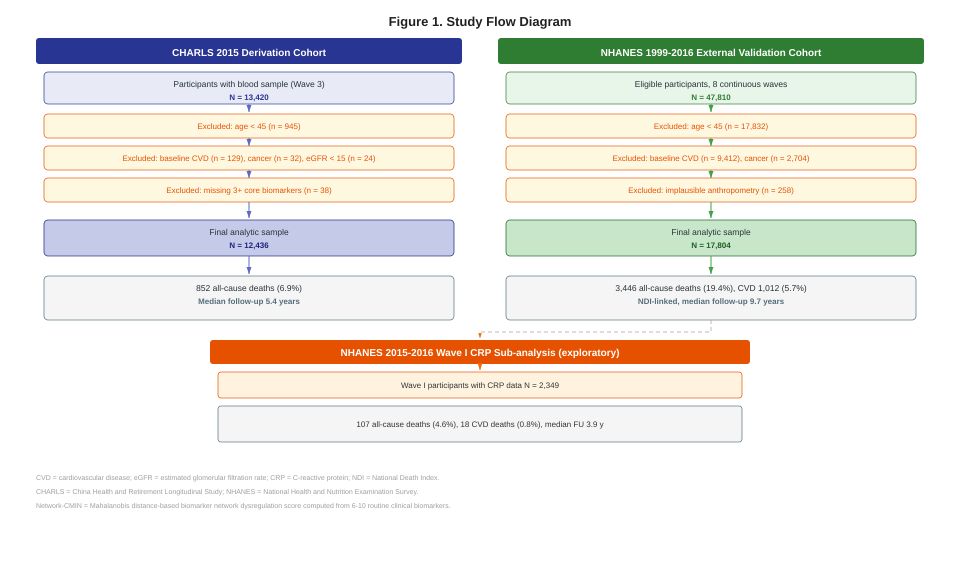
\includegraphics[width=\textwidth]{figures/fig1_strobe.pdf}
\caption{Study flow diagram. Left: CHARLS 2015 derivation cohort. Right: NHANES 1999--2016 external validation cohort. Bottom: NHANES 2015--2016 Wave I CRP sub-analysis.}
\label{fig:flow}
\end{figure}

\begin{figure}[h]
\centering
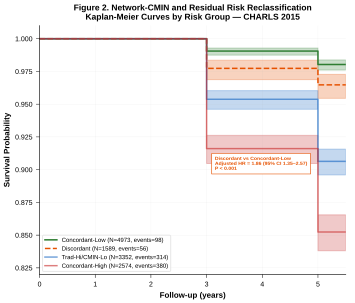
\includegraphics[width=0.85\textwidth]{figures/fig2_km_discordance.pdf}
\caption{Kaplan-Meier survival curves by four-group risk classification, CHARLS 2015 ($N = 12{,}436$). The Discordant group (low traditional risk, high Network-CMIN) had significantly elevated mortality relative to the Concordant-Low reference (adjusted HR, 1.86; 95\% CI, 1.35--2.57; $P < 0.001$).}
\label{fig:km}
\end{figure}

\begin{figure}[h]
\centering
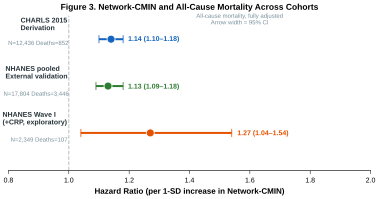
\includegraphics[width=0.9\textwidth]{figures/fig3_forest.pdf}
\caption{Network-CMIN and all-cause mortality across three cohorts. Hazard ratios are per 1-SD increase in Network-CMIN Z-score, adjusted for age, sex, and physical activity. Boxes are sized proportionally to the inverse variance. Error bars indicate 95\% confidence intervals.}
\label{fig:forest}
\end{figure}

\begin{figure}[h]
\centering
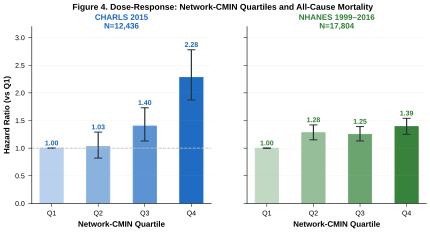
\includegraphics[width=\textwidth]{figures/fig4_doseresponse.pdf}
\caption{Dose-response relationship between Network-CMIN quartiles and all-cause mortality. Left: CHARLS 2015 derivation cohort (10 markers). Right: NHANES 1999--2016 validation cohort (6 markers). Reference category is Quartile 1. Error bars represent 95\% confidence intervals.}
\label{fig:dr}
\end{figure}

\newpage
% ============================================================
% SUPPLEMENTARY MATERIALS
% ============================================================

\section*{Supplementary Materials}

\subsection*{Figure S1. Kaplan-Meier curves by risk group in the NHANES pooled cohort}
\begin{figure}[h]
\centering
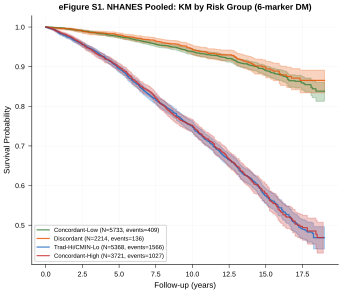
\includegraphics[width=0.85\textwidth]{figures/efigS1_nhanes_km.pdf}
\caption{Kaplan-Meier curves for the four-group risk classification in the NHANES 1999--2016 pooled cohort using the 6-marker Network-CMIN.}
\end{figure}

\subsection*{Figure S2. Distribution of Network-CMIN Z-scores}
\begin{figure}[h]
\centering
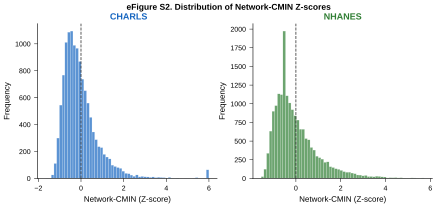
\includegraphics[width=\textwidth]{figures/efigS2_dm_distribution.pdf}
\caption{Distribution of Network-CMIN Z-scores in CHARLS 2015 (left) and NHANES 1999--2016 (right).}
\end{figure}

\subsection*{eTable S3. Within-CHARLS harmonization: Network-CMIN performance by biomarker set size}
\begin{table}[h]
\centering
\footnotesize
\caption{Association of Network-CMIN with all-cause mortality in CHARLS 2015 using different biomarker sets ($N = 12{,}488$, 848 deaths)}
\begin{tabular}{lp{5.2cm}cc}
\toprule
Biomarker set & Markers included & HR (95\% CI) & C-index \\
\midrule
10-marker (full) & CRP, glucose, HbA1c, TC, TG, HDL, LDL, SBP, DBP, BMI & 1.19 (1.14--1.24) & 0.785 \\
7-marker (Wave I equiv.) & CRP, glucose, TC, HDL, creatinine, SBP, DBP, BMI & 1.17 (1.13--1.22) & 0.784 \\
6-marker (pooled equiv.) & TC, HDL, creatinine, SBP, DBP, BMI & 1.12 (1.08--1.18) & 0.781 \\
\bottomrule
\multicolumn{4}{p{14cm}}{\footnotesize All models adjusted for age, sex, and physical activity. The 6-marker set, matching the NHANES pooled analysis, produced a 5\% attenuation in HR versus the full 10-marker set, supporting the NHANES 6-marker HR (1.13) as a conservative estimate. DM reference populations were defined separately for each marker set using identical clinical criteria.} \\
\end{tabular}
\end{table}

\clearpage
% ============================================================
% DECLARATIONS
% ============================================================

\section*{Declarations}

\subsection*{Ethics approval and consent to participate}
This study used secondary analysis of publicly available, de-identified population survey data and was exempt from institutional review board approval. CHARLS was approved by the Biomedical Ethics Review Committee of Peking University. NHANES was approved by the National Center for Health Statistics Research Ethics Review Board. All participants provided informed consent at the time of original data collection.

\subsection*{Consent for publication}
Not applicable.

\subsection*{Availability of data and materials}
CHARLS 2015 data are publicly available from the CHARLS project at Peking University (http://charls.pku.edu.cn/) after user registration and acceptance of a data use agreement. NHANES 1999--2016 data are publicly available from the National Center for Health Statistics (https://wwwn.cdc.gov/nchs/nhanes/). NHANES Public-Use Linked Mortality Files (follow-up through December 31, 2019) were obtained from the NCHS Data Linkage program (https://www.cdc.gov/nchs/data-linkage/mortality-public.htm). All analysis code (Python 3.12) is publicly available at https://github.com/CHI9-SATR/github{\_}repo.

\subsection*{Competing interests}
The authors declare that they have no competing interests.

\subsection*{Funding}
This research received no specific grant from any funding agency in the public, commercial, or not-for-profit sectors.

\subsection*{Authors' contributions}
Qingsong Gong conceived and designed the study, performed the statistical analysis, interpreted the results, and drafted the manuscript. Yuzhi Fan, Sixuan Shao, Xiaohan Li, and Yajing Du contributed to data acquisition, literature review, and critical revision of the manuscript. Qingping Guo supervised the study, provided clinical interpretation, and approved the final version for submission. All authors read and approved the final manuscript.

\subsection*{Acknowledgements}
We thank the China Health and Retirement Longitudinal Study (CHARLS) team at Peking University for collecting and disseminating the CHARLS data, and the National Center for Health Statistics (NCHS) for the NHANES data and linked mortality files. The analysis in this study used Python 3.12 with pandas, numpy, scipy, and lifelines; we acknowledge the open-source developers of these tools.

\clearpage
% ============================================================
\bibliographystyle{unsrtnat}
\bibliography{references_verified}
% ============================================================

\end{document}
